\documentclass[a4paper,10pt]{article}
% -----------------------------------------------------------
\usepackage[top=0.55in, bottom=0.25in, left=0.45in, right=0.75in]{geometry}
\usepackage{graphicx}
\usepackage{url}
\usepackage[super]{nth}
\usepackage{palatino}
\usepackage{tabularx}
\usepackage{graphicx}
\usepackage{wrapfig}
\fontfamily{SansSerif}
\selectfont

\usepackage[T1]{fontenc}
\usepackage
% [ansinew]
[utf8]
{inputenc}

\usepackage{color}
\definecolor{mygrey}{gray}{0.75}
\textheight=9.75in
\raggedbottom

\setlength{\tabcolsep}{0in}
\newcommand{\isep}{-2 pt}
\newcommand{\lsep}{-0.5cm}
\newcommand{\psep}{-0.6cm}
\renewcommand{\labelitemii}{$\circ$}

\pagestyle{empty}
% -----------------------------------------------------------
% Custom commands
\newcommand{\resitem}[1]{\item #1 \vspace{-2pt}}
\newcommand{\resheading}[1]{{\small \colorbox{mygrey}{\begin{minipage}{0.975\textwidth}{\textbf{#1 \vphantom{p\^{E}}}}\end{minipage}}}}
\newcommand{\ressubheading}[3]{
  \begin{tabular*}{6.62in}{l @{\extracolsep{\fill}} r}
    \textsc{{\textbf{#1}}} & \textsc{\textit{[#2]}} \\
  \end{tabular*}\vspace{-8pt}}
% -----------------------------------------------------------

\begin{document}
\hspace{0.5cm}\\[-0.2cm]
% \vspace{-5mm}
\vspace{-14mm}
\begin{wrapfigure}{r}{0.14\textwidth} 
    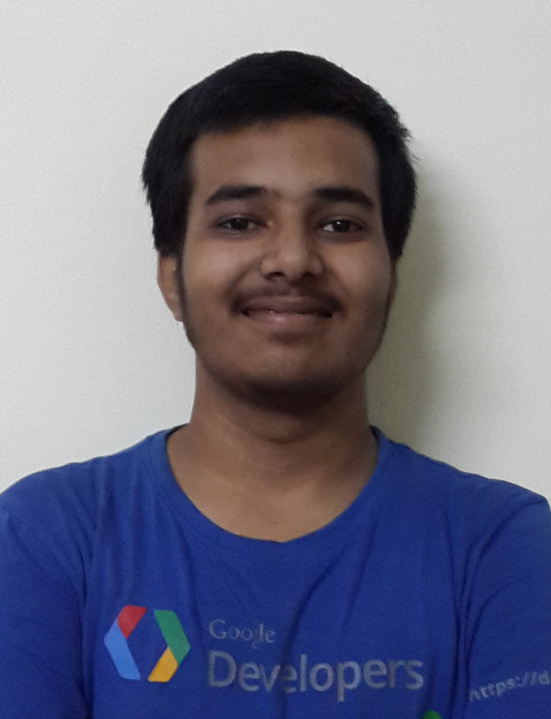
\includegraphics[width=0.15\textwidth]{photo}
\end{wrapfigure} \\\\

{\huge Nishant Gupta} \\ % \vspace{2mm}
\indent Third Year Student, \\
\indent Computer Science and Engineering, IIT Kanpur \\
\indent {I-307/5,IIT Kanpur, U. P., 208016} \\
\indent Mobile No.: \textit{7275726006} \\
\indent Email-id : \textit{nishgu@iitk.ac.in}  \\
\vspace{-1mm}
\hspace{4mm}\resheading{\textbf{ACADEMIC DETAILS} }\\[\lsep]
\\ \vspace{-2mm}
% \begin{table}[ht!]
\begin{center}
  \indent \begin{tabular}{ l @{\hskip 0.15in} l @{\hskip 0.15in} l @{\hskip 0.15in} l @{\hskip 0.15in} l }
            \textbf{Examination}  & \textbf{Institute} & \textbf{Year} & \textbf{CPI/\%} \\
            2017 (expected) & {B.Tech,  Computer Science} & IIT Kanpur  & 9.2/10.0  \\ 
            2013 & {HSCE} & Shivpuri Public School,Ashoknagar & 			93.60\%	\\
            2011 & AISSCE & Tara Sadan School,Ashoknagar  & 9.6/10.0   \\
          \end{tabular}
        \end{center}
        % \end{table}
\vspace{-0.5mm}
\hspace{4mm}        \resheading{\textbf{SCHOLASTIC ACHIEVEMENTS} }\\[\lsep]
        \begin{itemize} \itemsep -2pt
        \item
          Awarded \textbf{Academic Excellence Award} (IITK) given to top 5\% students on the basis of academic performance.
        \item
          Secured \textbf{AIR-248} out of 0.15
          million shortlisted  students in JEE-Advanced 2013.
        \item
          Qualified \textbf{Regional Mathematical Olympiad}(Rajasthan Region).
        \end{itemize}

        \resheading{\textbf{TECHNICAL SKILLS} }\\[\lsep]
        \begin{itemize}
        \item \noindent \textbf{Languages} (C, C++, Java, dart, Javascript, Haskell,
          Scala, x86 Assembly(AT\&T Syntax)),\textbf{Database} (MySQL) \textbf{Script}
          (Python, Shell), \textbf{Tools} (git, Angular, Android App Development, sbt,
          gradle, cabal).
        \end{itemize}

        \resheading{\textbf{INTERNSHIPS} }\\[\lsep]
        \begin{itemize}
        \item \textbf{  Altisource Business Solutions}(Technology Intern) \hfill  \textit{May'15-Jul'15}
          \vspace{-2mm}
          \begin{itemize} \itemsep -2pt
          \item Worked on the projects \textbf{Actor Equivalence and Identity Stitching} and \textbf{Event Data Clustering}
            for the company's consumer analytics product `Pointilist'
          \item Designed an algorithm for solving the actor equivalence problem
            (Established a relation between actors and streaming events) for
            single Multiple platforms.
          \item Built a generic
            framework that takes varying
            Consumer data from
            different tenants and
            Processes, normalizes and
            Clusters it to derive
            meaningful inferences.
          \end{itemize}
        \end{itemize}

        \resheading{\textbf{KEY PROJECTS} }\\[\lsep]
        \begin{itemize} \itemsep -1mm
        \item
          \textbf{Online Web Platform} - \textit{Under Prof. Manindra Agarwal}
          \hfill \textit{Nov'14-Present}
          \vspace{-2mm}\begin{itemize} \itemsep -2pt
\item Implemented Google Drive
          Integration and various
          small features for a web platform
          that uses \textbf{Dart} on front-end
          and \textbf{Scala} on back-end. 
\item Designed and developed the frontend using bleeding edge frameworks like AngularDart, Polymer, etc 
\item Currently
          developing Android app for
          same web platform.
\end{itemize}
        \item  \textbf{Sentiment Analysis of Social Media} - {\footnotesize
            Takneek'14 }   \hfill \textit{ Aug'14
}          \vspace{-2mm}\begin{itemize} \itemsep -2pt
          \item Application developed during Web-Dev, Takneek'14 and secured \textbf{\nth{1}} position.
          \item Provided an interface to analyse the past and present social sentiment of brands and their products.
          \item  Identify `good' and `bad' features of the product and suggest weak points to improve it.
          \end{itemize}
        \item
          \textbf{Image Trianglization} - \textit{ Programming Club, IIT Kanpur }                  \hfill \textit{Jun'14-Jul'14}
          \vspace{-2mm}\begin{itemize}  \itemsep -2pt
          \item Renders image using only triangles and gives the sense of image.
          \item Uses \textbf{OpenCV} for Image Processing and Manipulation,
            Tkinter for GUI and webcam support.
          \item Uses Delaunay Triangulation so that image is aesthetically pleasing.
          \end{itemize}
        \item
          \textbf{News Map} - \textit{ ACA, IIT Kanpur }
          \hfill  \textit{Feb'14-Apr'14}
          \vspace{-2mm}\begin{itemize} \itemsep -2pt
          \item A webapp that plots news on a world map  using various APIs for location resolution, news fetching and map plotting.
          \end{itemize}
        \end{itemize}

        \resheading{\textbf{RELEVANT COURSEWORK} }\\[\lsep] \vspace{2mm}
        \begin{itemize}
\item[]
                                        \begin{tabular}{p{69mm}@{\hskip 0.25in} p{80mm}} 
                                          CS210 - Data Structures and Algorithms(\textbf{A*}) & CS201 - Discrete Mathematics(\textbf{A})  \\
                                          CS345 - Algorithms II(*)             & MSO201 - Probability and Statistics(\textbf{A}) \\
                                          CS653 -Functional Programming(*)  & \hfill * - Ongoing
                                        \end{tabular}

        \end{itemize}

\vspace{-1mm}
        \resheading{\textbf{POSITIONS OF RESPONSIBILITY} }\\[\lsep] \vspace{1mm}
                                                   \begin{itemize} \itemsep -2pt
                                                  \item \textit{Seceretary} of Programming Club, IIT Kanpur. \hfill \textit{2014-2015}
                                                    \vspace{-2mm}\begin{itemize}
                                                      \item Part of a team of 15 members made to manage the activities of the Programming Club, IITK
                                                      \item Mentored freshmen for various Programming club competitions.
                                                      \end{itemize}
                                                      \item \textit{Co-ordinator},
                                                        Funzone, Udhghosh'14 -
                                                        Annual Inter-College
                                                        Sports Fest of
                                                        IIT-Kanpur. \hfill \textit{Sep'2014}
                                                    \end{itemize}
      \end{document}

